\section{Taylor's Theorem}

$ f(x) = f(c) + \frac{f'(c)}{1!} (x-c)^1 + \dots + \frac{f^{(n)}(c)}{n!}(x-c)^n + \frac{f^{(n+1)}(\xi)}{(n+1)!}(x-c)^{(n+1)} $,

i.e. $f(x) = \sum_{k=0}^n \frac{f^{(k)}(c)}{1!} (x-c)^k + \frac{f^{(n+1)}(\xi)}{(n+1)!}(x-c)^{(n+1)} $

, where $\xi$ is between $c$ and $x$ (either $c < x$ or $c > x$).

\subsection{Simple case of Taylor's Theorem}

Take $n = 1$, we have
$f(x) = f(c) + f'(c) (x - c) + O((x - c)^2)$.

By dropping the error term,
$f(x) = f(c) + f'(c) (x - c)$,\\
which is the equation of tangent line at $x = c$.

\subsection{Lagrange's Mean Value Theorem}

$ f(x) - f(c) = f'(\xi)(x-c) $\\
$\rightarrow \frac{f(x)-f(c)}{x-c} = f'(\xi)$ (Lagrange's Mean Value Theorem)

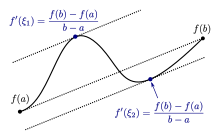
\includegraphics{MVT.png}

i.e. there is at last one point $\xi$, where slope of tangent line at $\xi$ = slope of straight line joining $(x, f(x))$ and $(c, f(c)) $.

Assumption 1: $f(t)$ is continuous in $[x, c]$. \textbf{(Closed interval!)}\\
Assumption 2: $f'(t)$ exists in $(x, c)$. \textbf{(Open interval is enough.)}

\begin{quote}
    We require $f(t)$ be continuous in $[x, c]$ as we have to apply extreme value theorem.
\end{quote}

\subsection{Before Proving Lagrange's Mean Value Theorem}

To prove Lagrange's Mean Value Theorem, we need to ``deep'' theorems about continuous functions. One of them is Intermediate Value Theorem (IVT).

\subsubsection{Intermediate Value Theorem}

Let $f(x)$ be continuous in $[a, b]$. Then for every $v$ between $f(a)$ and $f(b)$, there is a value $t$ in $[a, b]$ such that $f(t) = v$.

\textbf{Specific application:}

Let $f(x)$ be continuous in $[a, b]$ and $f(a) \cdot f(b) < 0$. Then there exists at least one $\xi \in [a, b]$ such that $f(\xi) = 0$.

\textbf{Example:}

Let $f(x) = x^3 + 3x - 2$. As $f(0) = -2$ and $f(1) = 2$, there is a root for $f(x) = 0$ in $[0, 1]$. (We can apply bisection method to approximate the root.)

\subsubsection{Extreme Value Theorem}

Let $f(x)$ be continuous in $[a, b]$. Then there exists global maximum $M$ and global minimum $m$ and $x_M, x_m \in [a, b]$,\\
such that $f(x_M) = M \geq f(x)$ and $f(x_m) = m \leq f(x)$ for all $x \in [a, b]$.

\subsubsection{Rolle's Theorem}

For any function $f(x)$ that is continuous in $[a, b]$, $f'(x)$ exists in $(a, b)$, and $f(a) = f(b)$,\\
there exists $\xi \in [a, b]$ such that $f'(\xi) = 0$.

\subsubsection{Cauchy's Mean Value Theorem}

Let $f(x), g(x)$ be both continuous in $[a, b]$ and $f'(x), g'(x)$ both exist in $(a, b)$. Also $g'(x) \not = 0$ in $[a, b]$. (i.e. $g'(x)$ is either increasing or decreasing.)

Then we have

$$\frac{g(b) - g(a)}{f(b) - f(a)} = \frac{f'(\xi)}{g'(\xi)}$$

for some $\xi \in [a, b]$.

\subsection{Proof of Lagrange's Mean Value Theorem}

First we prove Rolle's Theorem. Then we use it to prove Cauchy's Mean Value Theorem.

Lagrange's Mean Value Theorem is the application of Cauchy's Mean Value Theorem on $g(x) = x$. 

\subsubsection{Proving Cauchy's Mean Value Theorem from Rolle's Theorem}

Produce a function $\Phi(x)$ satisfying $\Phi(a) = \Phi(b)$.

Rearranging Cauchy's Mean Value Theorem, we have

$$ (f(b) - f(a)) g'(\xi) - (g(b) - g(a)) f'(\xi) = 0 $$

This motivates us to let that

$$ \Phi(x) = (f(b) - f(a)) g(x) - (g(b) - g(a)) f(x) $$

We can check that $\Phi(a) = -f(a)g(b) + f(b)g(a)$ and $\Phi(b) = -f(a)g(b) + f(b)g(a)$. Hence $\Phi(a) = \Phi(b)$.

Also $\Phi(x)$ is differentiable as it is a linear combination of $f(x)$ and $g(x)$.

Applying Rolle's Theorem to $\Phi(x)$, we have

$$ \frac{d\Phi(x)}{dx}|_{x=\xi} = \frac{d}{dx}[ (f(b) - f(a)) g(x) - (g(b) - g(a))f(x) ] $$

which is equal to $(f(b) - f(a)) g'(\xi) - (g(b) - g(a)) f'(\xi)$.

Hence

$$ \frac{f(b) - f(a)}{g(b) - g(a)} = \frac{f'(\xi)}{g'(\xi)} $$

\subsection{Discussion on continuity}

$f(x)$ is continuous at $c$ if $\lim_{t\to c} f(x) = f(c)$.

Similar to limit of a function, you can add, subtract, multiply and divide continuous functions.

$f(t) \oplus g(t)$ is continuous at $t = a$, where $\oplus$ is $+$, $-$, $\times$ or $\div$.\\
(When $\oplus$ is $\div$, $g(a)$ must not be 0.)

If $g(t)$ is continuous at $t = a$, and $f(u)$ is continuous at $t = g(a)$,\\
then $f(g(t))$ is continuous at $t = a$.

\begin{quote}
    e.g. $\sqrt{1+e^t}$ is a composite function, where
        $f(u) = \sqrt{u}$ and $g(t) = 1 + e^t$.
\end{quote}

\subsection{Application of Lagrange's Mean Value Theorem}

Show $|\sin x - \sin y| \leq |x - y|$.

\textbf{Proof:}

Rewrite the question so that $\frac{|\sin x - \sin y|}{|x - y|} \leq 1$.

Let $f(t) = sin(t)$ be defined on $[x, y]$.\\
$$\frac{f(y) - f(x)}{y - x} = \frac{\sin y - \sin x}{y - x}$$
By Lagrange's Mean Value Theorem, this is equal to $f'(\xi) = \cos \xi$.\\
As $\cos\xi \in [-1, 1]$, $|\cos\xi| \leq 1$, and this is proved.